\section{Conclusions}

The queries selected for this project were pretty different from each other, and each of them asked for a different optimization technique.

This said, we can have a comprehensive look at what happened to execution times of all the queries given all the techniques analyzed.

If we compare this behavior with the comprehensive size of the dataset, we can have a more critical opinion on what can be the best technique to adopt in our case.

\begin{figure}[h!] 
\centering 
\begin{minipage}{0.5\textwidth} 
\centering 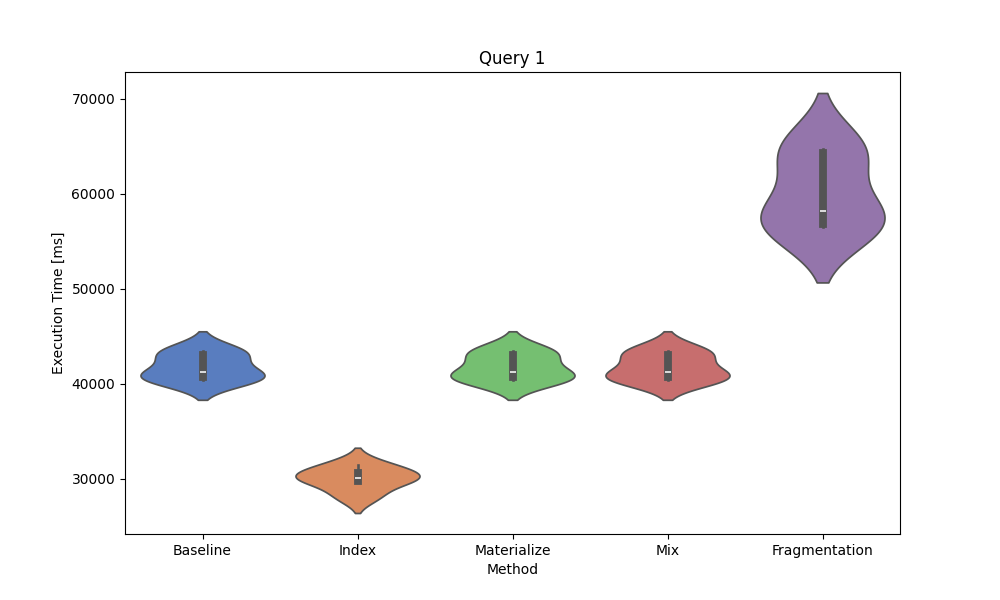
\includegraphics[width=\linewidth]{images/query1.png}  
\end{minipage}
\begin{minipage}{0.45\textwidth} 
\centering 
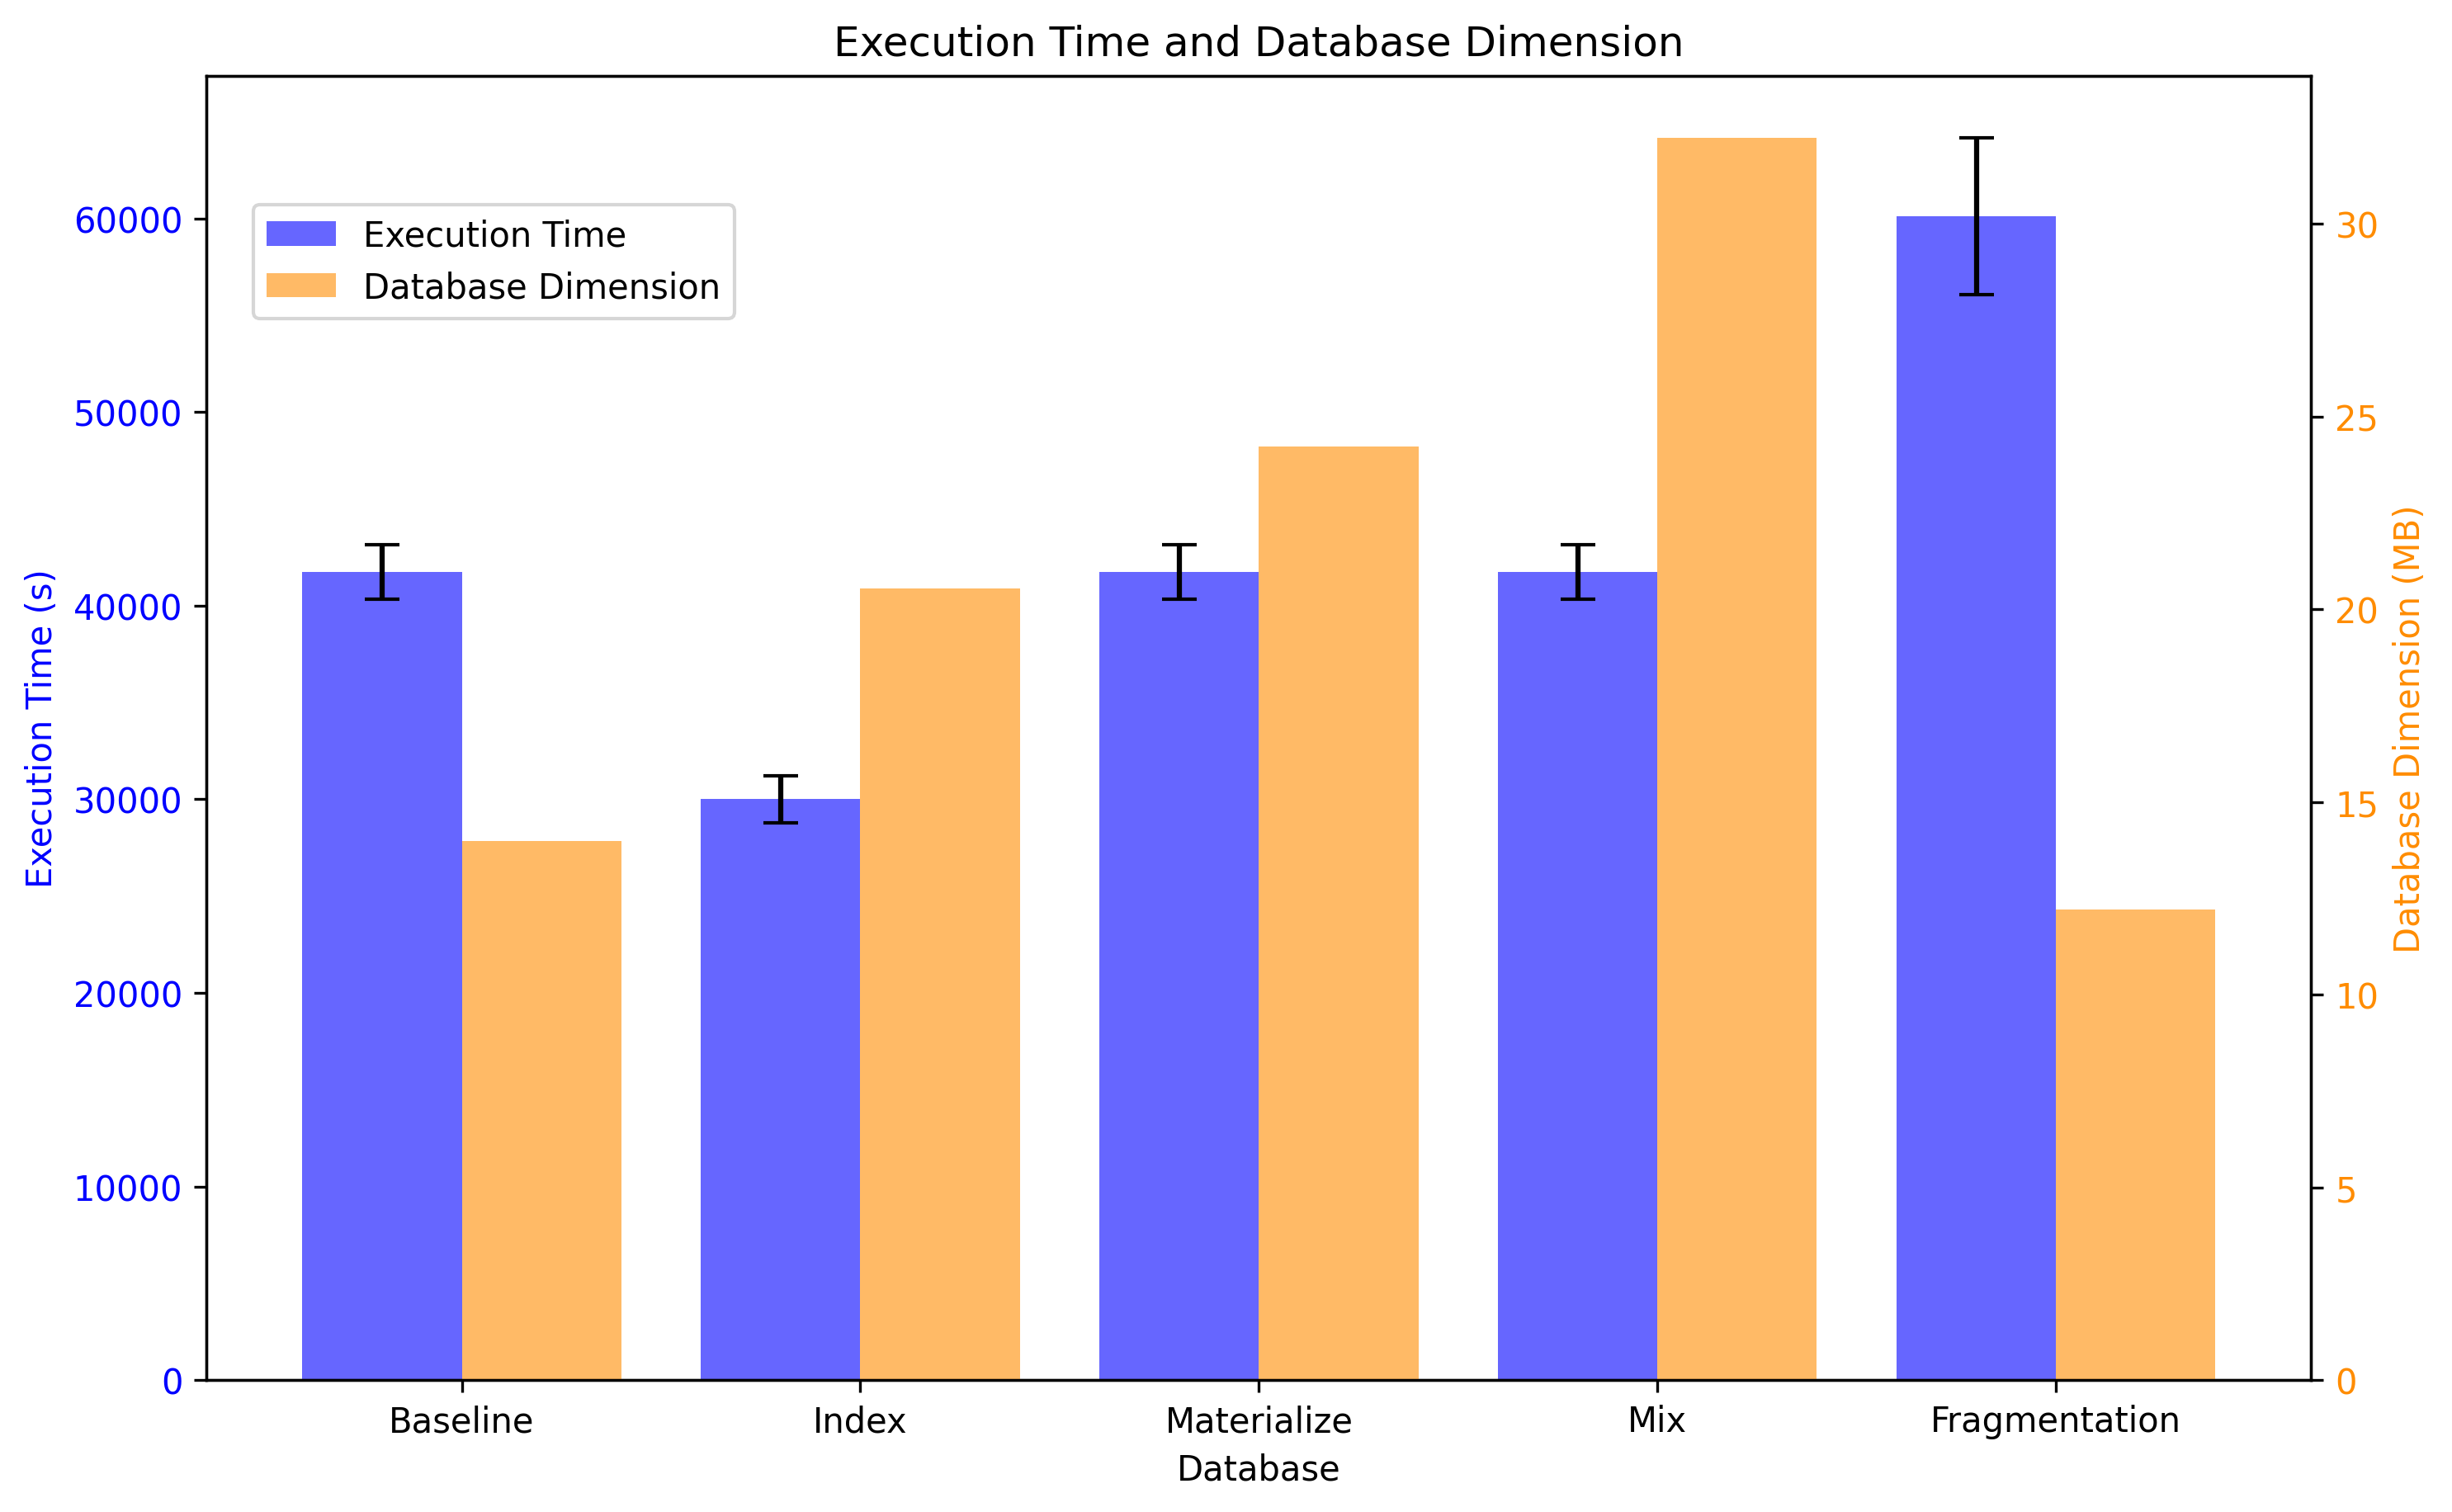
\includegraphics[width=\linewidth]{images/double_barplot_q1.png} 
\end{minipage} 
\caption{Query 1} 
\end{figure}

Regarding query one we can see that the most significant improvement is reached with the usage of indexing. We can notice also that the fragmentation of the lineitem table worsen the performances, leading to an execution time higher than the one of the baseline. This may be expected since the slicing condition is highly non selective, and scanning (almost) all the tables in the partition have an higher cost than scanning the same quantity of rows in a single table.
The performances with the strategy of materialization didn't change since the materialized views are not involved in this query.

\begin{figure}[h!] 
\centering 
\begin{minipage}{0.5\textwidth} 
\centering 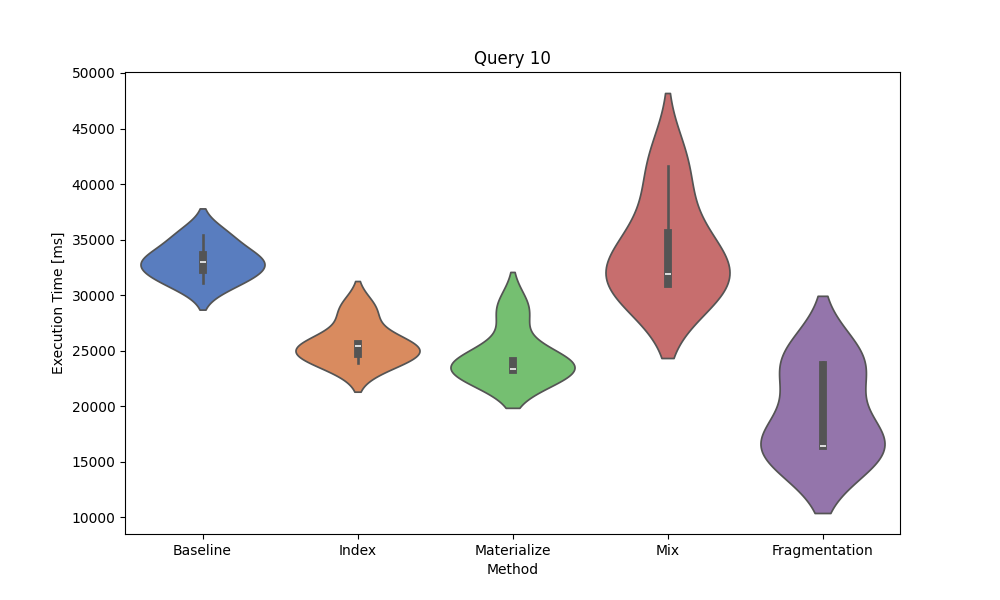
\includegraphics[width=\linewidth]{images/query10.png}  
\end{minipage}
\begin{minipage}{0.45\textwidth} 
\centering 
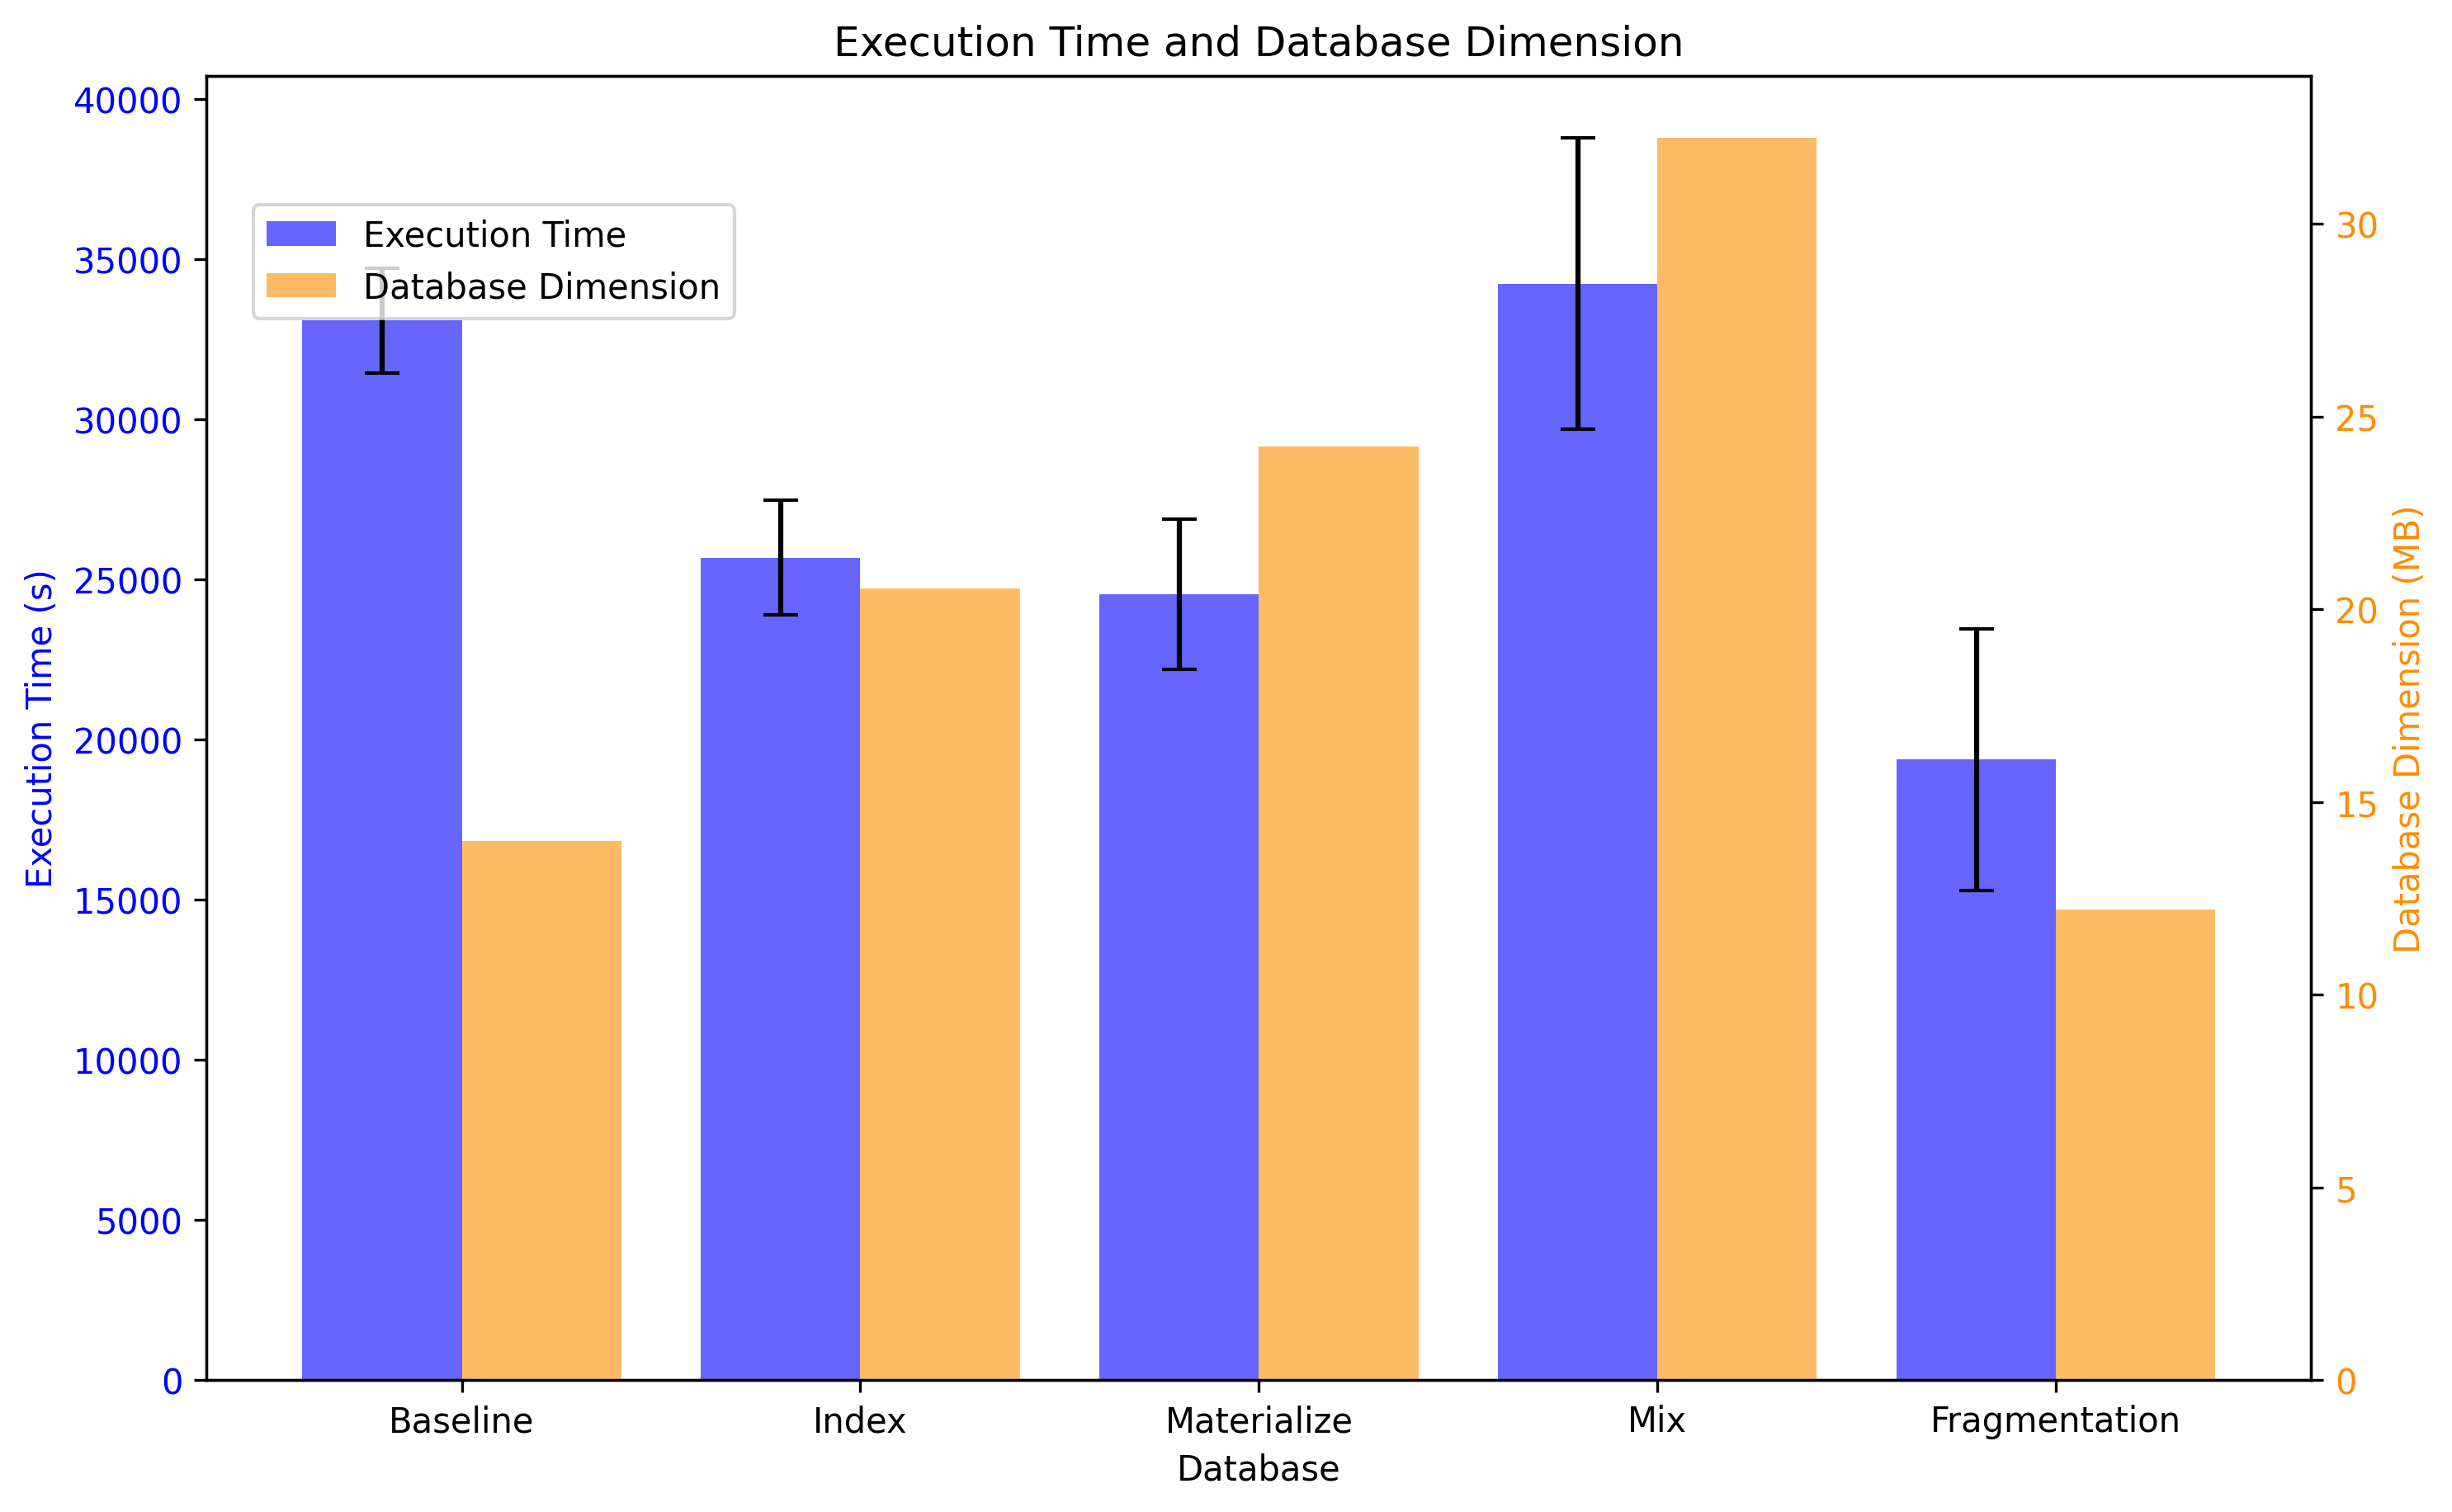
\includegraphics[width=\linewidth]{images/double_barplot_q10.png} 
\end{minipage} 
\caption{Query 10} 
\end{figure}

Regarding query 10 we can see that the performances of all the approaches are comparable, with a slight improvement given by the fragmentation. Indeed the fragmentation on orderdate is fully exploited by the slicing condition that involved a three month linespan. Given this consideration it may be expected an even bigger improvement, but the scan of the lineitem partition to retrieve the subpartition with "l\_returnflag=R" moderated the gains.

\begin{figure}[h!] 
\centering 
\begin{minipage}{0.5\textwidth} 
\centering 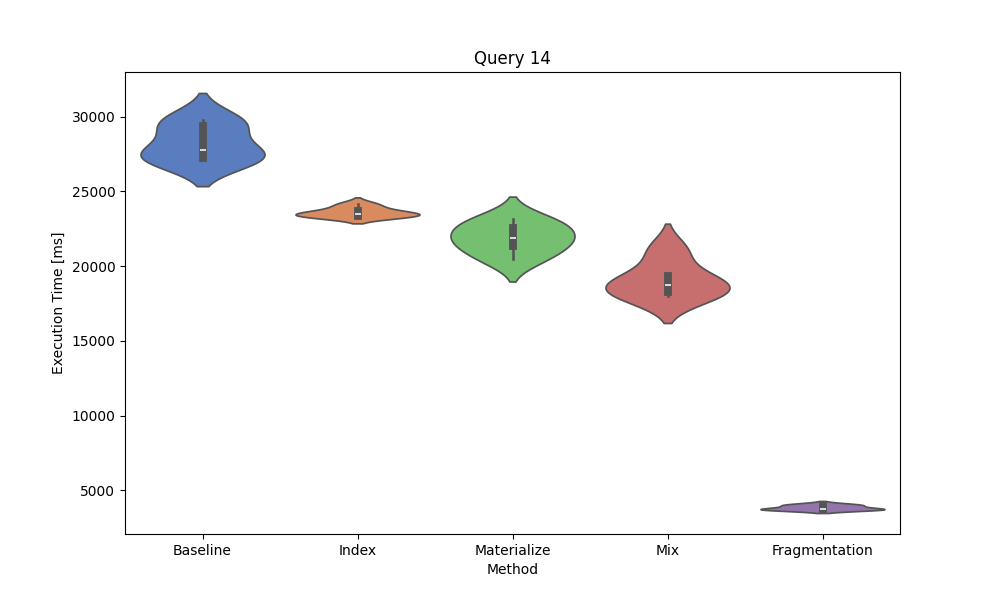
\includegraphics[width=\linewidth]{images/query14.png}  
\end{minipage}
\begin{minipage}{0.45\textwidth} 
\centering 
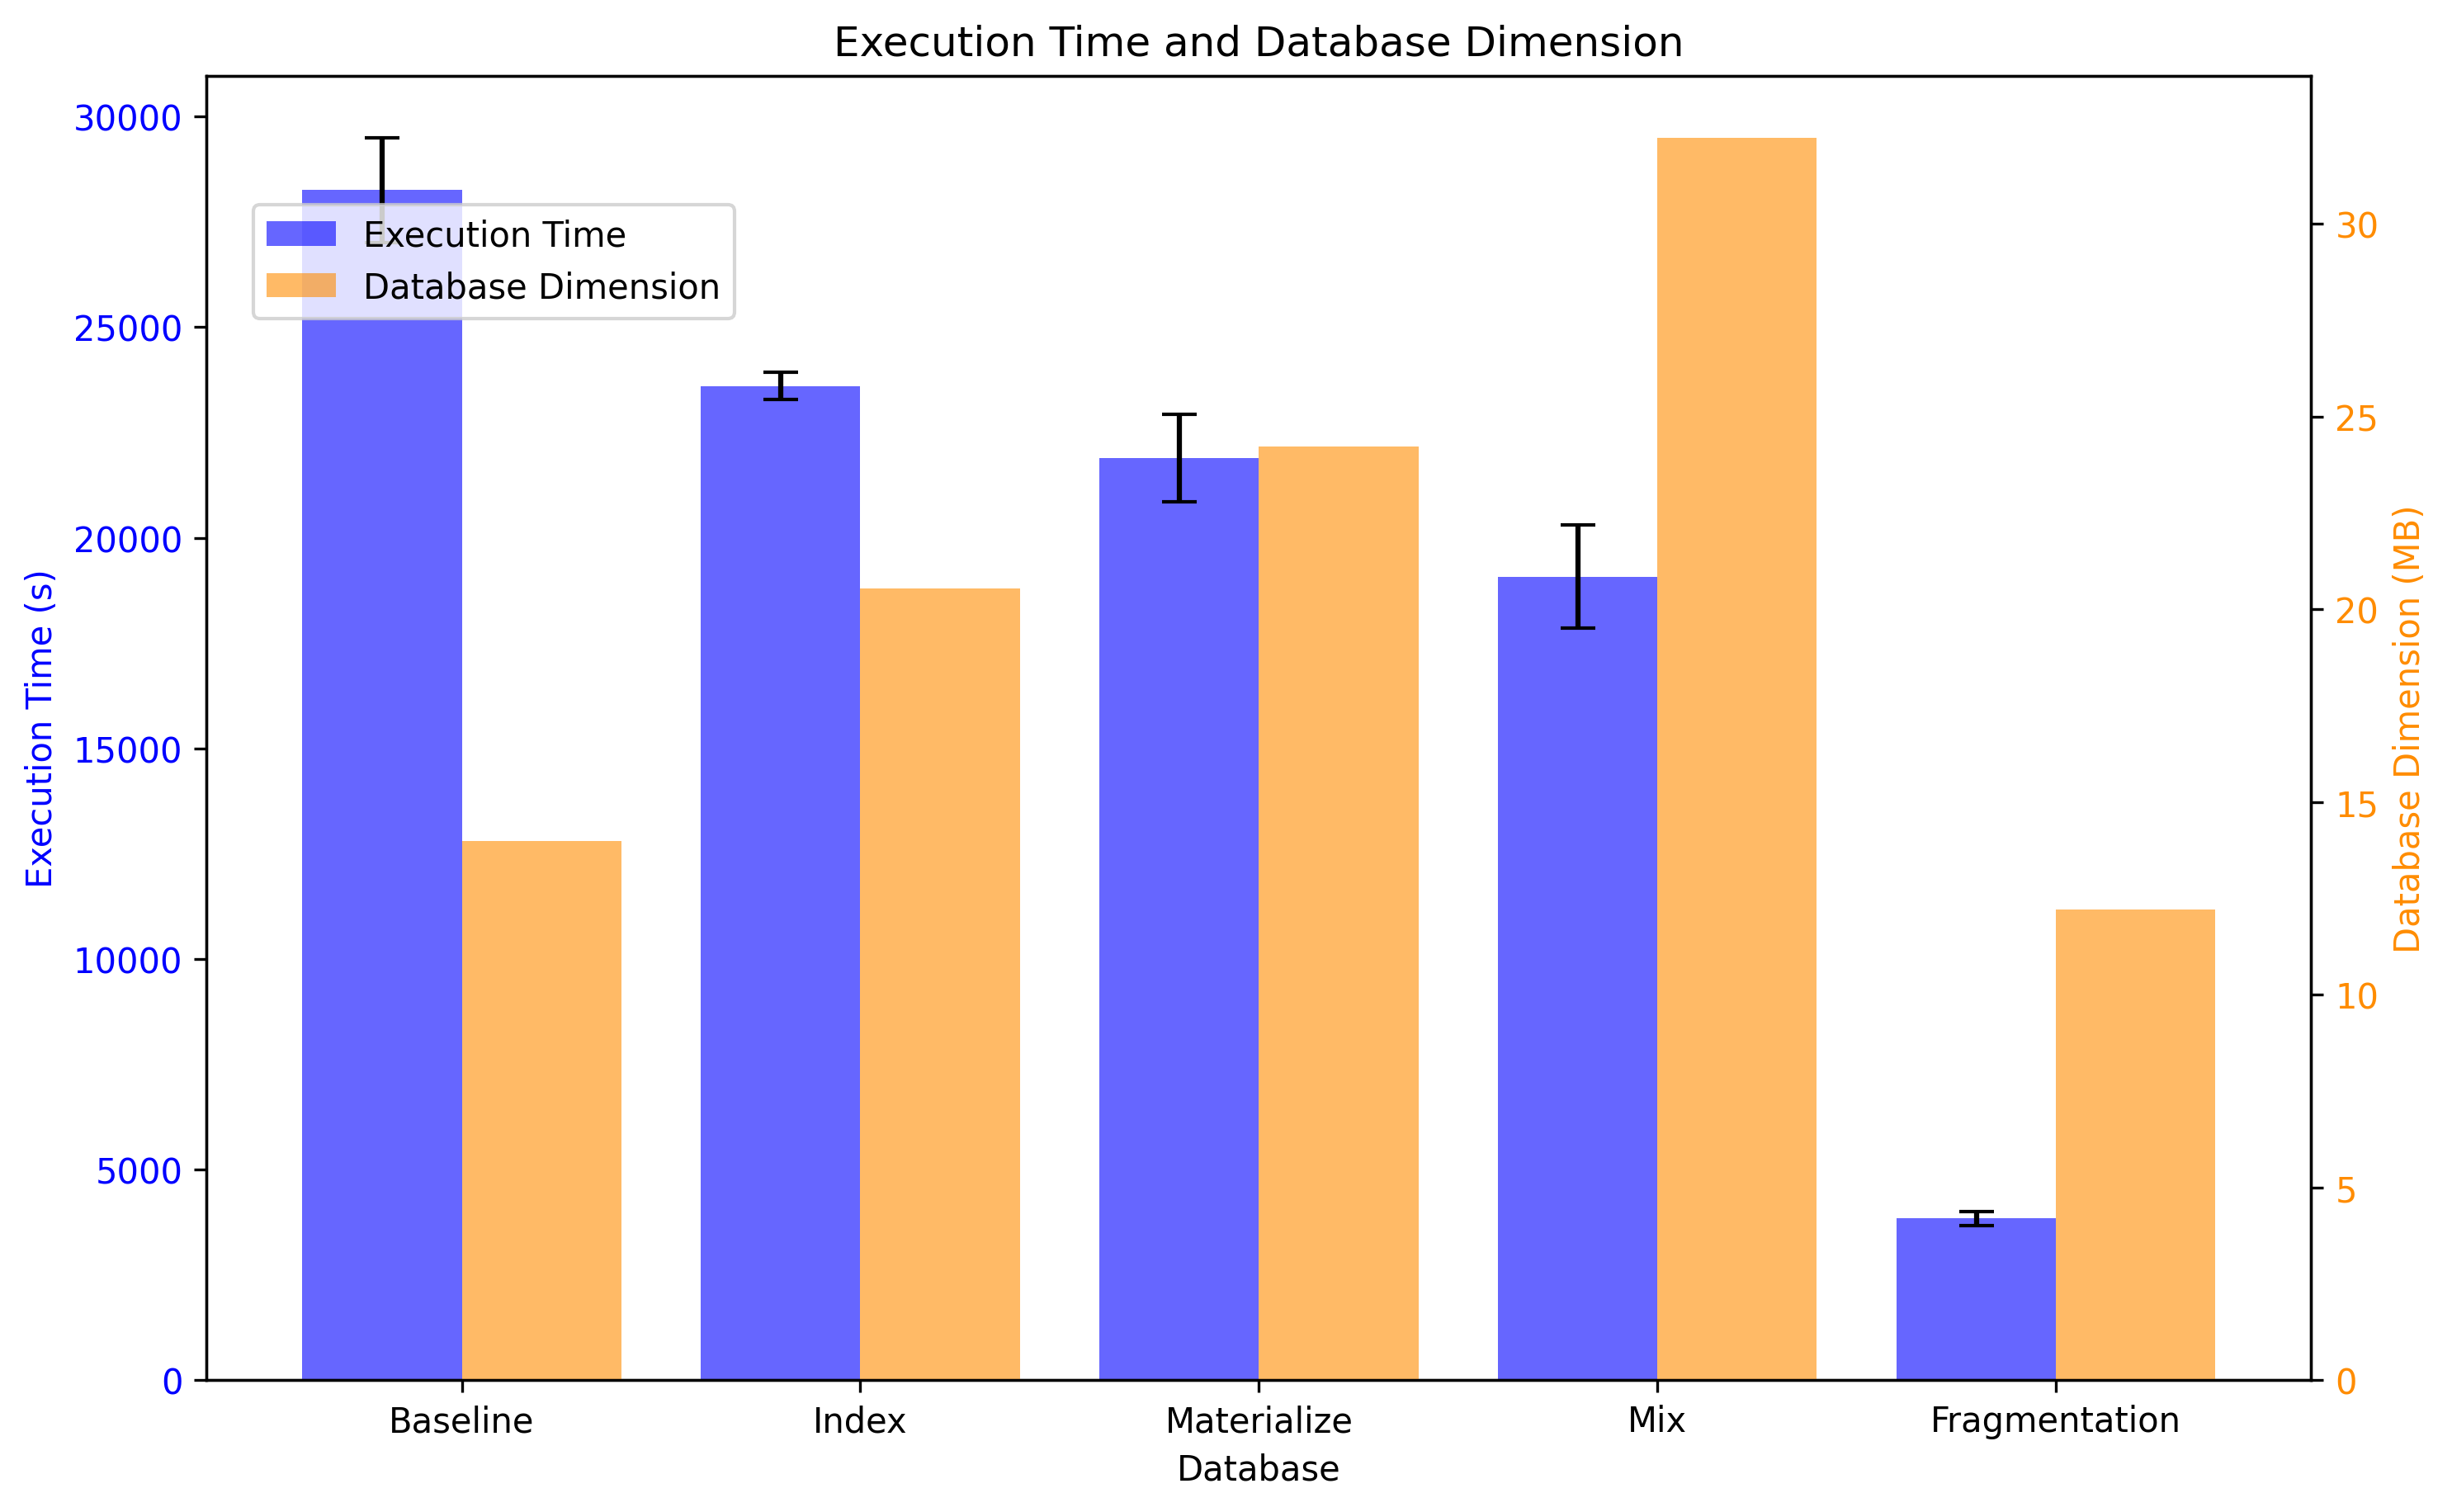
\includegraphics[width=\linewidth]{images/double_barplot_q14.png} 
\end{minipage} 
\caption{Query 14} 
\end{figure}

Query 14 is the one that obtained the most evident improvement with the fragmentation. This is explained by the fact that the lineitem table is the most computationally expensive to be scanned, by indroducing the fragmentation on l\_shipdate, the DBMS needs to consider only one subtable, furthermore the group by condition is facilitated by the subpartition on l\_returnflag.
\begin{figure}[h!] 
\centering 
\begin{minipage}{0.5\textwidth} 
\centering 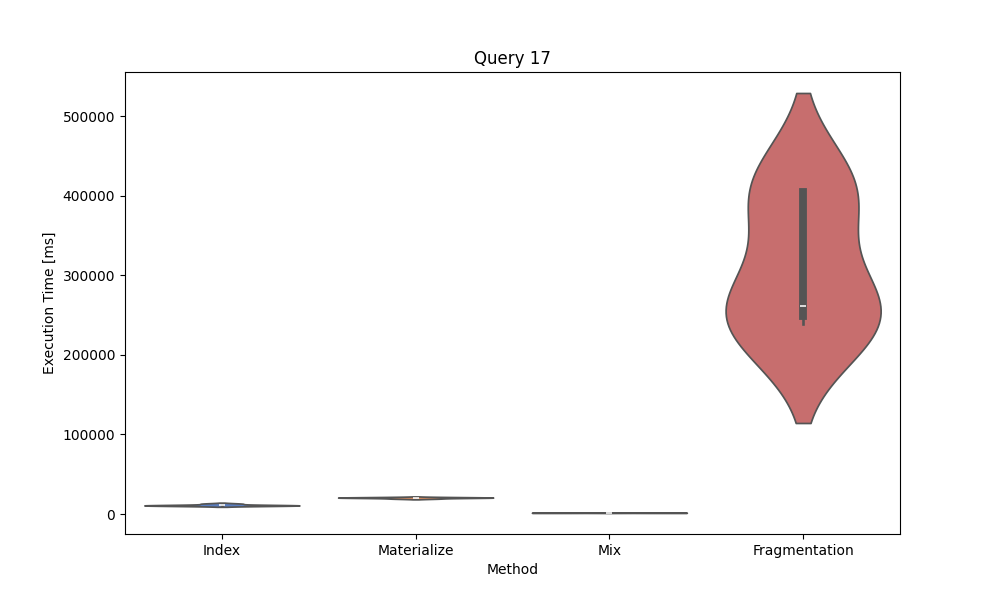
\includegraphics[width=\linewidth]{images/query17.png}  
\end{minipage}
\begin{minipage}{0.45\textwidth} 
\centering 
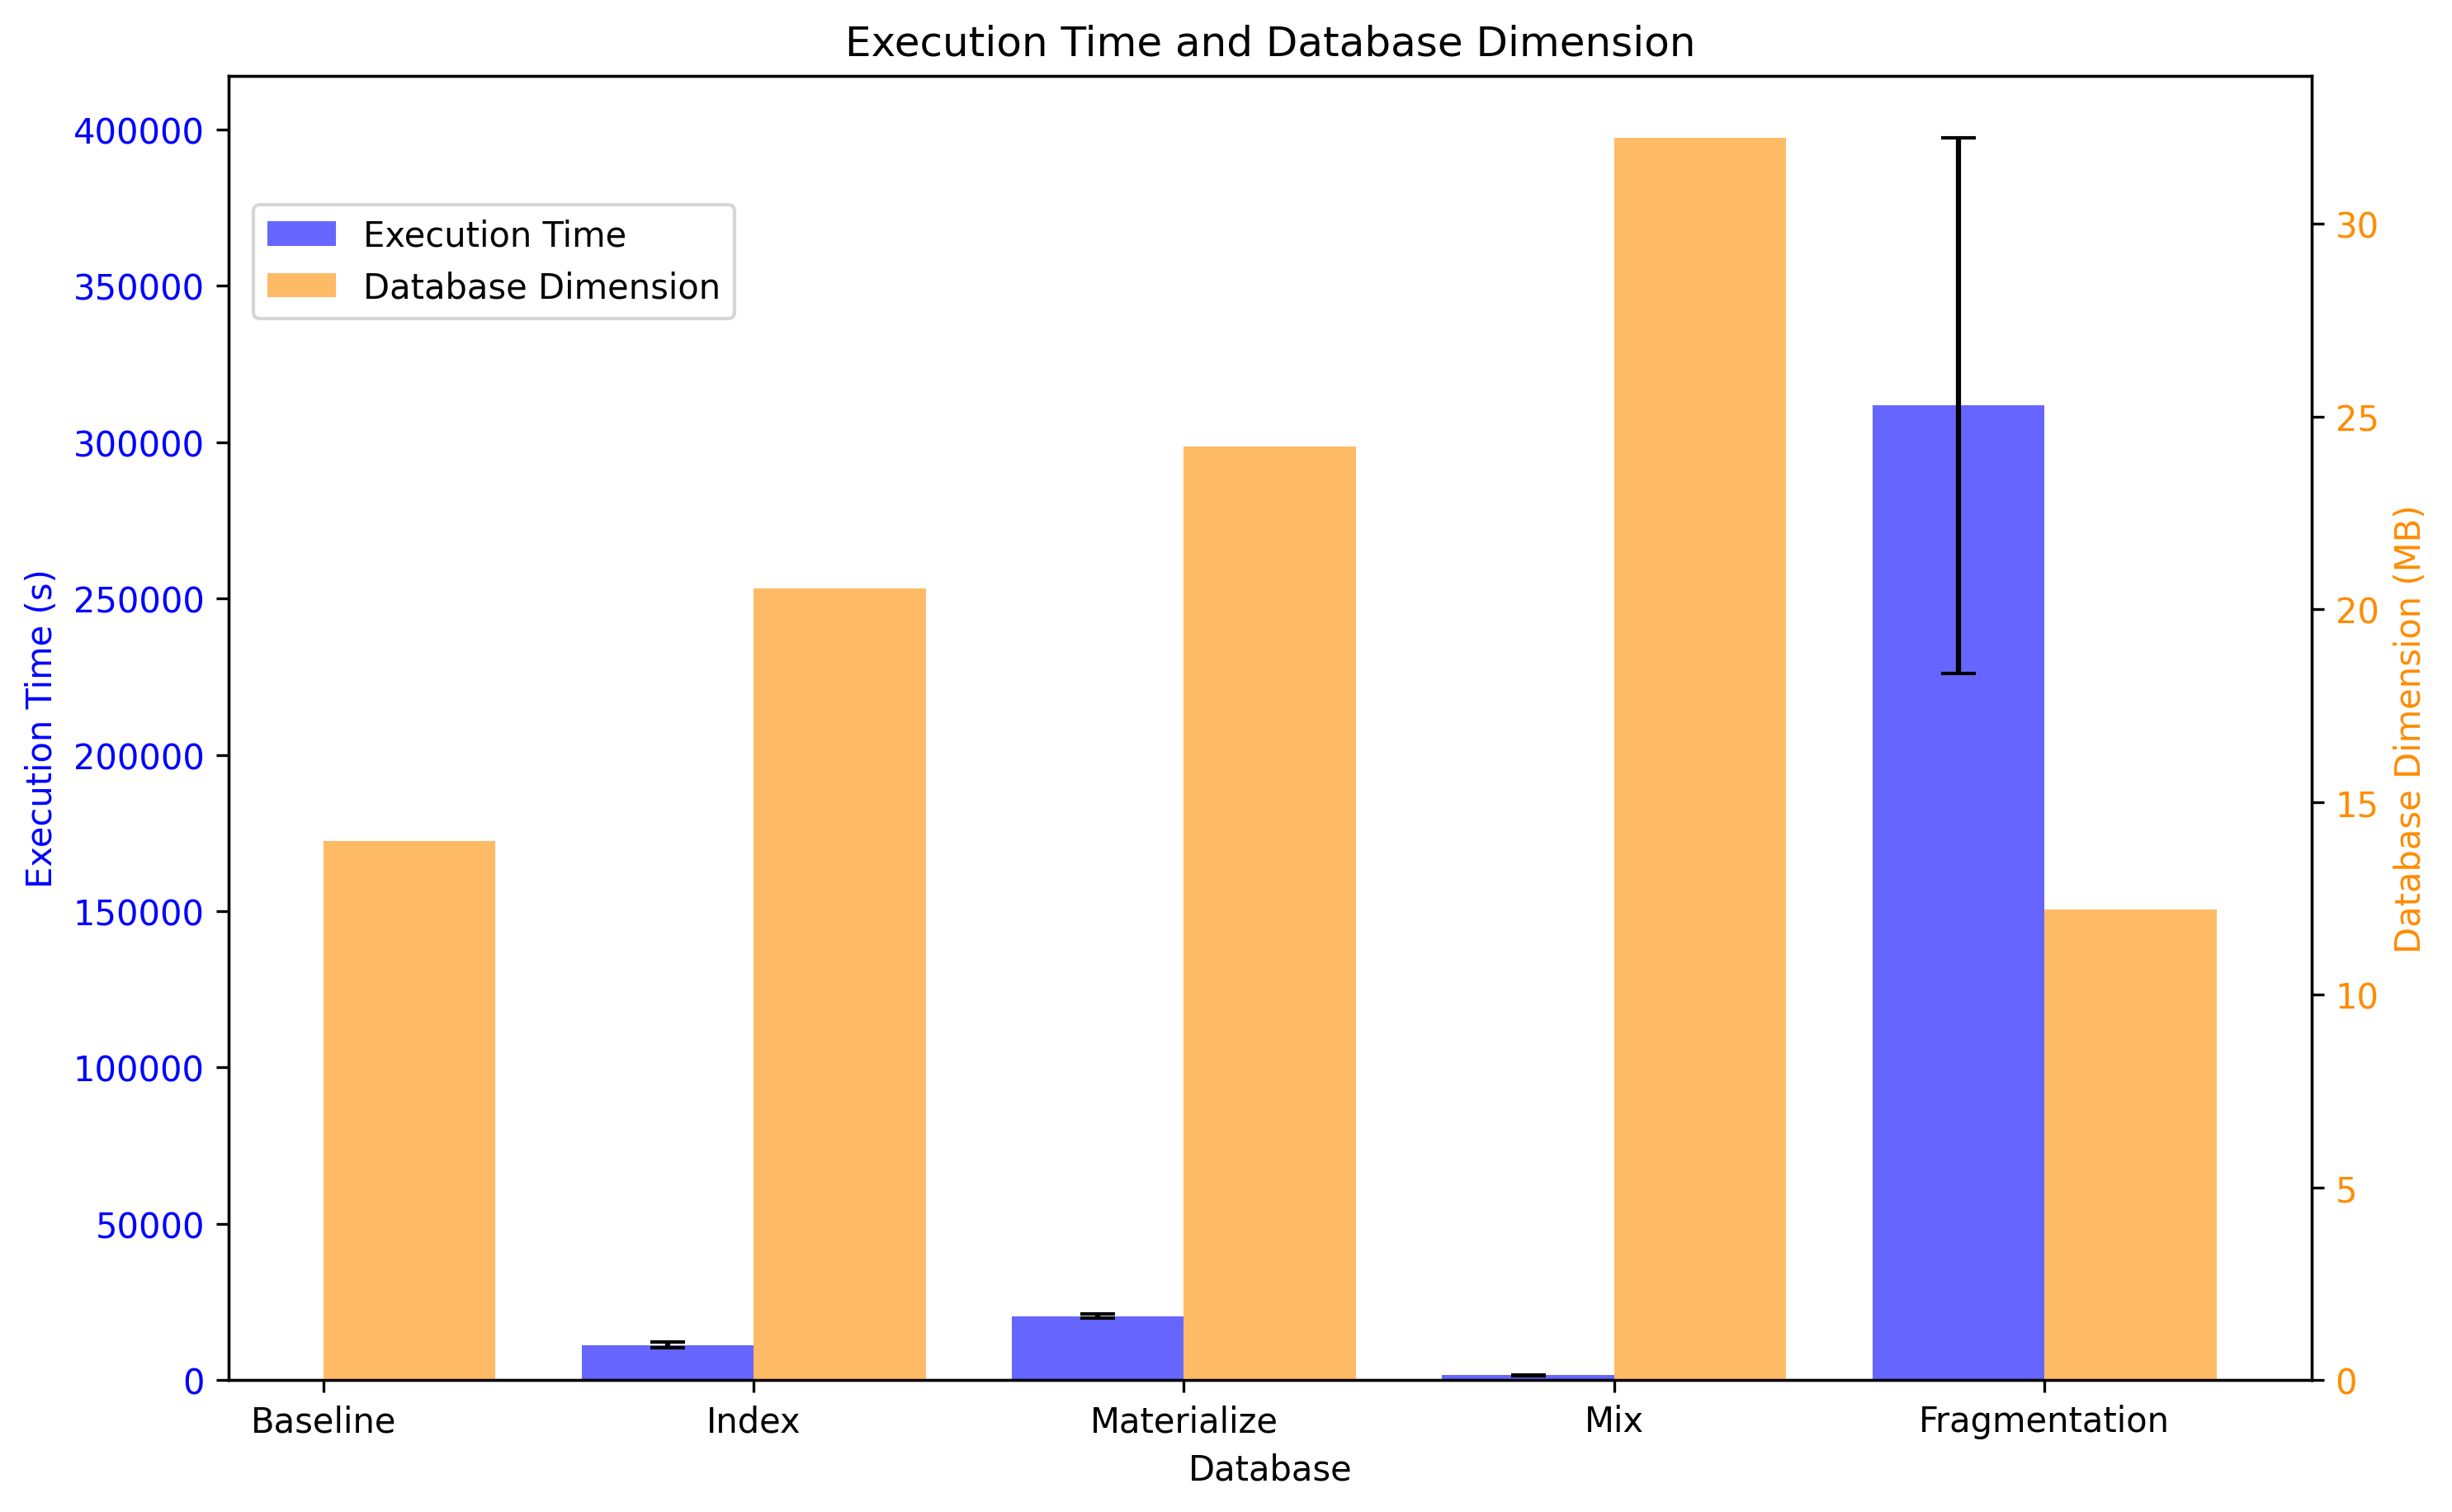
\includegraphics[width=\linewidth]{images/double_barplot_q17.png} 
\end{minipage} 
\caption{Query 17} 
\end{figure}

Regarding query 17 all the proposed form of optimization significantly improved the execution time with respect to the baseline (in principle with an execution time greater than 2 hours). A mixed approach of materialization and indexed allows to perform the slicing in a really efficient way, without having to perform the join at every execution since it's included in the pre-computed view.  

As a general overview of this project we observe that a combination of different types of optimization is the best way to improve the performances of different queries. Also we can consider that sometimes it is important to find a balance between the benefits that a technique may carry in speeding up the computation, and the space (in term of memory) that this technique may require. Also it is important to average the effect of an optimization technique over different types of queries to avoid introducing too specific tools/procedures(?)
[Supercazzola finale una volta che abbiamo i risultati]